\chapter{\label{chapter:PropagatorStates}The State Vector and State Management}
\chapauthor{Darrel J. Conway}{Thinking Systems, Inc.}

GMAT supplies a class, the GmatState, which provides a low level container for mission related
state information manipulated by the system during a simulation.  The GmatState is populated with
data from the objects in GMAT's current model so that the code that implements the processes in the
simulation can act on the data in a generic fashion.  The synchronization between the data that
is manipulated and the objects that supply these data is handled by classes derived from the
StateManager class.  These interactions are described at a high level in this chapter.  Specific
uses of the state vector and managers can be found in the chapters describing propagation
(Chapter~\ref{chapter:PropagatorOverview}) and orbit determination
(Chapter~\ref{chapter:EstimationOverview}).

\section{Design Motivation and Overview}

The combination of one or more GmatState objects and one or more associated StateManagers as
implemented in GMAT follows the Mediator design pattern.  The GmatState acts as an object
that accumulates data from the elements of GMAT's mission into a format that can be used by the
algorithms that manipulate these data to run a mission.  Once these algorithms complete their work,
the changed data in the GmatState object is then passed back to the objects representing physical
entities in the model.  The coordination of the GmatState with the objects providing the state data
is handled by an instance of a class derived from the StateManager class.

GMAT uses this intermediary to keep the propagation and estimation processes as generic as
possible.  In GMAT, the propagation algorithms work by advancing an arbitrarily sized vector of
numbers over time.  Knowledge about the way these numbers evolve is all predefined when the
propagators are set up prior to the actual evolution.  This predefined setup and subsequent
application of the propagation algorithm streamlines the process of changing the state of GMAT's
objects as the model epoch changes.  It also makes the definition of the propagation vector
flexible and extensible.  New elements that need to evolve over time can be added to GMAT's
propagation subsystem by defining an ID for the new propagation type, supplying the corresponding
evolution providers (for instance, a PhysicalModel defining ordinary differential equations used
to integrate the new element), and changes making this new element visible to the propagation
enabled commands.

Similarly, in GMAT estimation is constructed to apply an estimation algorithm to an arbitrarily
sized vector of numbers.  The connection between the state vector used in the estimation process and
the objects defined in GMAT's mission is made when the estimation subsystem is initialized.  The
synchronization of data between the estimation vector and the mission obects is managed by an
instance of a class derived from the StateManager class.  This abstraction of the estimation state
vector from the mission defined objects is used to keep the estiamtion subsystem extensible and
flexible in the same way as is provided for the propagation subsystem.

An added feature of this design is that any other algorithms that work on a vector of numbers
and an associated epoch can use GMAT's objects to build this generic data set simply by deriving a
new StateManager appropriate to the algorithm and using that StateManager to handle the data
interchange between the state vector and the associated GMAT objects.  Implementors that need such
new capablities in GMAT need only study the patterns implemented in the estimation and propagation
subsystems in order gain insight into how to extend GMAT for these new capabilities.

\subsection[A Propagation State Example]{An Example: State and State Management in Propagation}

You can see an example of this mediation\footnote{A more detailed look at the objects and
interactions in this example can be found in Section~\ref{section:PropagationExample}.  This
section is intended to illustrate how the objects, state and state manager operate in the context
of the example mission.} in GMAT's propagation subsystem. Consider a mission consisting of two
spacecraft that are propagated for a day using a Runge-Kutta integrator and a force model consisting
of a 4x4 geopotential model, point mass effects from the Sun and Moon, solar radiation pressure, and
atmospheric drag modeled using the MSISE-90 atmosphere model.  In GMAT, the user configures four
objects to model this system: two spacecraft, an ODEModel that holds the force model, and a
Runge-Kutta integrator.  The mission control sequence that uses these objects is a single Propagate
command.  Ignoring the details of the object configuration, the setup for this mission can be
scripted:

\begin{quote}
\texttt{Create Spacecraft sat1 sat2\\
\\
Create ForceModel fm\\
Create Propagator prop\\
prop.FM = fm\\
\\
\% The Mission Control Sequence\\
Propagate prop(sat1, sat2) \{sat1.ElapsedDays = 1.0\}}
\end{quote}

\noindent From the perspective of the state vetor and manager, the behavior required by this
scripting can be broken into four phases followed by GMAT's propagation subsystem when running a
mission: (1) Script Parsing, (2) Initialization in the Sandbox, (3) Final Preparation before
propagation, and (4) Propagation.  (The fifth phase in the life of a propagation enabled
command, command finalization, does not have a direct affect on the state and state manager
elements in this script.)  The following paragraphs provide an overview of how state and the state
manager behave in each of these phases.

\begin{enumerate}
\item \textbf{Script Parsing}  During script parsing, all four of the resources in the script --
two spacecraft, the force model, and the PropSetup -- are created and placed in GMAT's global
configuration.  Three of these resources contain GmatState members: each Spacecraft uses a
GmatState to hold the orbital state and epoch information, and the ODEModel (defined by the
ForceModel line) contains a GmatState pointer, which is not yet initialized.  The PropSetup defined
by the Propagator line contains an instance of the PropagationStateManager class, a subclass of
StateManager.  That PropagationStateManager, in turn, contains a GmatState object that will be used
by the PropSetup's propagator as the container for the raw data that gets propagated.

\item \textbf{Initialization}  When a run is started that uses these objects, GMAT clones each
object into the Sandbox used for the run.  That places a copy of the object, including each member
GmatState and PropagationStateManager, into the Sandbox's object store.  The objects in the object
store are then initialized.  As part of this process, object references that won't change because
of actions performed in the Mission Control Sequence are set.  For this script, the ODEModel
containing the force model is passed into PropSetup.  The PropSetup is initialized, but the
internal components -- the Propagator and, if applicable, ODEModel, are not yet initialized; that
piece of initialization is deferred until the next phase of the process.

Once the objects have been initialized, the Mission Control Sequence performs its initialization.
Each command is passed the Sandbox object stores (that is, the local object map and the global
object store) and the local solar system.  Each command is then issued an instttruction to perform
its initialization.  For our example, the only command in the Mission Control Sequence is a
Propagate command.  On initialization, this command retrieves the PropSetup it needs and clones it
for use by the command.  This cloning makes copies of the Propagator and (if set) the ODEModel.
The Propagate command then locates each of the other referenced objects it uses.  It passes the
objects calling for propagation (in this case, sat1 and sat2) into the PropagationStateManager
associated with the PropSetup.  Once these objects have been set, the command initializes the
PropagationStateManager by calling the methods that build the state vector and associate the
objects with the elements of that vector.  The resulting state is passed to the local ODEModel,
completing the part of the command initialization concerned with the state vector and state manager.

\item \textbf{Preparation for Propagation}  The final step that occurs prior to propagation updates
the elements involved in propagation to capture changes that may have occurred from previous
events in the Mission Control Sequence, and then retrieves the current data for the state vector
from the objects.  During this phase, the ODEModel uses the PropagationStateManager to construct the
mapping between elements of the state vector and the components of the ODEModel that supply
derivative information for integration.  During this phase in initialization, the Propagator and
ODEModel themselves get initialized.

\item \textbf{Propagation}  In many ways the actual propagation phase is the simplest of those
described here.  GMAT's propagators evolve the state vector using the coded propagation algorithm.
Each time a propagation step completes, a call is made to the PropagationStateManager to update the
affected objects with the propagated data.  Occasionally -- for example, while evaluating stopping
conditions -- the propagator backs out a step by requesting a refresh from the
PropagationStateManager.
\end{enumerate}

The details of each of the steps described above can be found in
Chapter~\ref{chapter:PropagatorOverview}.  The following sections describe the GmatState and
StateManager classes.


\section{The GmatState Class}

The GmatState is a helper class designed for processes that need a general purpose vector of real
number data, an epoch for those data, and information that lets the process decode the data in a
meaningful way.  GMAT uses instances of the GmatState class in the Spacecraft class to store the
epoch and orbital elements for each spacecraft, in the propagation subsystem to store the data that
evolved over time in the simunation, and in the estimation subsystem for the estimation state
vector.  The GmatState can be used as a standalone entity, or on conjuction with a StateManager.

Each element of the GmatState can have properties associated with it that provide information about
the type of data in that element.  These ancillary data include an identifier for the data type,
a text string that describes the data member in a dot-delimited format, and an index pointing to
other data in the state vector associated with the element.  An example of the settings for these
data can be found by looking at the layout of the Cartesian state data for a spacecraft in the
vector assembled by the PropagationStateManager prior to propagation.  Table~\ref{table:GmatState}
shows this layout for a spacecraft named sat.

\begin{table}
\begin{center}
% use packages: array
\begin{tabular}{llll}
\textbf{theData} & \textbf{dataID} & \textbf{dataType} & \textbf{associate} \\
7100.0 & 3700 & sat.CartesianState.1 & 0 \\
0.0 & 3700 & sat.CartesianState.2 & 0 \\
1000.0 & 3700 & sat.CartesianState.3 & 0 \\
0.0 & 3700 & sat.CartesianState.4 & 0 \\
7.35 & 3700 & sat.CartesianState.5 & 0 \\
1.0 & 3700 & sat.CartesianState.6 & 0
\end{tabular}
\end{center}
\caption[GmatState for Propagation]{\label{table:GmatState}GmatState for a Spacecraft as seen in
Propagation}
\end{table}

\subsection{GmatState Attributes}

\begin{itemize}
\item\textbf{GmatEpoch theEpoch} The epoch of the state data managed by the GmatState.  GMAT
requires that all such state data in a GmatState use the same epoch.
\item\textbf{Real *theData} The state data.
\item\textbf{Integer *dataIDs}  The id associated with the state data.
\item\textbf{Integer *associatedElements}  The index of the first element associated with each
element.
\item\textbf{StringArray dataTypes}  Text descriptors of the elements.
\item\textbf{Integer stateSize} Total number of elements that are in the state.

\end{itemize}

\subsection{GmatState Methods}

\begin{itemize}
\item\textbf{Real\& operator[](const Integer index)}  Sets an element of the state vector.
\item\textbf{Real operator[](const Integer index) const}  Reads an element of the state vector.
\item\textbf{void SetSize(const Integer size)}  Resizes the state vector to a new size.
\item\textbf{Integer GetSize() const} Retrieves the current size of the state vector.
\item\textbf{Real* GetState()}  Retrieves the state vector.  This method provides direct access to
the entire state vector.  It is used to enhance performance over that provided by element-by-element
access methods.
\item\textbf{bool SetState(const Real *data, const Integer size, const Integer start = 0)}  Sets
all or part of the state vector to new values.  The new data is input through the data inputn
parameter, which is a vector of length given by the size parameter.  These data are written into
the state vector starting at the element specified by the start parameter.  The method traps writes
that would exceeed the valid range for the state vector.
\item\textbf{GmatEpoch GetEpoch() const}  Retrieves the epoch.
\item\textbf{GmatEpoch SetEpoch(const GmatEpoch ep)}  Sets the epoch.
\item\textbf{bool SetElementProperties(const Integer index, const Integer id, const std::string
\&textId, const Integer associate)}
\item\textbf{const StringArray\& GetElementDescriptions()}
\item\textbf{Integer GetAssociateIndex(const Integer id)}
\end{itemize}

\subsection{\label{section:GmatStateSetup}Representative Layouts for a GmatState}

\begin{figure}[htb]
\begin{center}
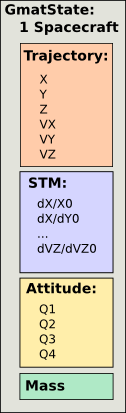
\includegraphics[63,207]{Images/PropVectorComponents.png}
\caption{\label{figure:PropVectorComponents}Representative Elements of a GmatState}
\end{center}
\end{figure}

Figure~\ref{figure:PropVectorComponents} shows a representative layout of the data in a GmatState
for a single spacecraft.  The vector displayed here is the GmatState used by a numerical
integrator that is modeling the evolution of the spacecraft's trajectory, state transition matrix,
and attitude during a finite burn maneuver.  When a PropagationStateManager assembles a GmatState,
it follows a set of ordering rules designed to make the data in the GmatState fall in a specific
order so that access from the propagators is simplified.  The general order, as shown in this
example, is to place trajectory data first in the vector, followed by associated matrices that
evolve along with the trajectory, then attitude data followed by associated attitde matrices, then
user defined elements, and finally transitory elements like mass, which only changes (through
propagation) during maneuvers.

\begin{figure}[htb]
\begin{center}
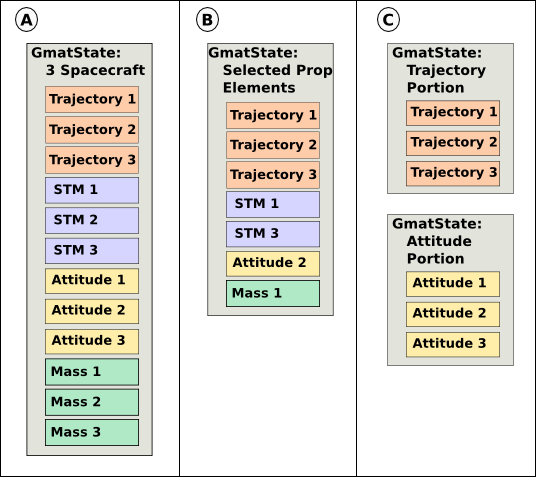
\includegraphics[268,239]{Images/ThreeStateVectors.png}
\caption[State Element Arrangement Examples]{\label{figure:ThreeSatPropVector}Element Arrangement
of a GmatState for Three Propagation Schemes}
\end{center}
\end{figure}

This ordering can be seen more explicitly in the subfigures of
Figure~\ref{figure:ThreeSatPropVector}.  In subfigure A, the GmatState shown is a vector constructed
for three spacecraft, where the mission needs to propagate the trajectory, state transition matrix,
and attitude for all three while maneuvering all three simultaneously.  Subfigure B shows another
example, where the propagation need not integrate every element of all of the spacecraft.  In this
example, the trajectory is integrated for all three spacecraft.  The state transition matrix is only
propagated for the first and third spacecraft, the attitude is propagated for the second, and the
first spacecraft is depleting mass during a maneuver.  Subfigure C shows a mixed mode propagation,
where the trajectory for our three spacecraft is propagated using a precalculated, ephemeris based
propagator and the attitude is propagated numerically.  Since there are two propagators involved in
this case, the state data is contained in two separate GmatStates.

\section{\label{section:StateManager}The StateManager Class}

The GmatState described above provides a container for state data so that algorithms that need to
work with that data can manipulate it in an abstract way, without direct knowledge of the objects
that supply the data.  The StateManager class hierarchy provides the tools that build GmatStates
and interface the new state objects to the objects supplying the data.  StateManagers are tailored
to the specific subsystems that contain them.  Examples of the subsystem StateManagers can be found
in the Propagation subsystem (Chapter~\ref{chapter:PropagatorOverview}) and the Estimation
subsystem (Chapter~\ref{chapter:EstimationOverview}).

The StateManager class hierarchy, including the propagation and estimation state managers, is shown
in Figure~\ref{figure:StateManagementClasses}.  The StateManager class defines some basic data
structures and interfaces shared by all state managers.  These elements are described in the
following sections.

\begin{figure}[htb]
\begin{center}
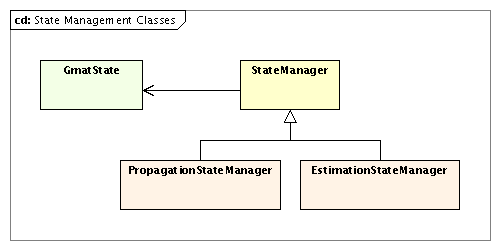
\includegraphics[250,125]{Images/StateManagementClasses.png}
\caption{\label{figure:StateManagementClasses}State Management Classes}
\end{center}
\end{figure}

\subsection{Attributes}

The StateManager base class contains the following member data elements:

\begin{itemize}
\item\textbf{Integer stateSize}:  The size required for the GmatState vector.
\item\textbf{GmatState state}:  The managed GmatState.
\item\textbf{ObjectArray objects}:  A vector of objects that supply data for the GmatState.
\item\textbf{std::vector<Integer> epochIDs}:  A vector of IDs on the objects used to validate epoch
data when the GmatState is manipulated.
\item\textbf{std::map<GmatBase*, StringArray*> elements}:  The mapping between objects and the
corresponding elements that they provide in the GmatState.
\item\textbf{GmatBase* current}:  A pointer to the most recently used object, provided for
convenience.
\end{itemize}

\subsection{Methods}

The StateManager class implements methods that define core state management capabilities, and
defines the interfaces for methods that must be implemented in the derived classes.  These methods
are described here:

\subsubsection{Implemented Methods}

\begin{itemize}
\item\textbf{virtual Integer GetCount(Gmat::StateElementId elementType = Gmat::UNKNOWN\_STATE)}:
Retrieves the number of objects that support the specified type.
\item\textbf{virtual bool UpdateState()}:  DEfines an interface for updating the state vector when
that vector cannot be updated by other means.  The default implenmentation has no affect.
\item\textbf{virtual GmatState* GetState()}:  Retrieves the GmatState managed by a StateManager
instance.
\item\textbf{virtual bool GetStateObjects(ObjectArray\& pObjects, Gmat::ObjectType type =
Gmat::UNKNOWN\_OBJECT)}:  Fills the input object array with pointers to the objects of the
specified type that supply data for the managed GmatState.
\end{itemize}

\subsection{Abstract Methods}

\begin{itemize}
\item\textbf{virtual bool SetObject(GmatBase* theObject) = 0}:  Adds an object to the list of
objects that supply data for the managed GmatState.
\item\textbf{virtual bool SetProperty(std::string propName) = 0}:  Sets the property string for an
element of the state vector.
\item\textbf{virtual bool BuildState() = 0}:  Assembles the GmatStaet vector from the current lists
of objects and properties.
\item\textbf{virtual bool MapObjectsToVector() = 0}:  Retrieves data from GMAT's objects and fills
these data into the GmatState vector.
\item\textbf{virtual bool MapVectorToObjects() = 0}:  Sets data on GMAT's objects based on the
contents of the GmatState vector.
\end{itemize}

\subsection{Enumerations used in State Management}

GMAT defines an enumeration, the StateElementId, which is used to identify the elements of the
state vector component by component.  This enumeration identifies the predefined component types
that a GmatStae can contain, and includes provisions for extending the element definition.  The
current set of element identifiers can be found in the file gmatdefs.hpp in the base/include
folder of GMAT's source code.  StateEleemntId is contained in the Gmat namespace.  The following
definitions can be found there at this writing:

\begin{itemize}
\item\textbf{UNKNOWN\_STATE = -1}:  Identifier if the element type is not known.
\item\textbf{CARTESIAN\_STATE = 3700}: The element is a member of the Cartesian state for an object.
\item\textbf{EQUINOCTIAL\_STATE}: The element is a member of the equinoctial state for an object.
\item\textbf{ORBIT\_STATE\_TRANSITION\_MATRIX}: The element is a member of the 6x6 orbit stae tra
nsition matrix for an object.
\item\textbf{MASS\_FLOW}: The element is the mass element used when mass is depleted from an object.
\item\textbf{PREDEFINED\_STATE\_MAX}: The identifier for the end of the predefined portion of the
enumeration.
\item\textbf{USER\_DEFINED\_BEGIN = 3800}:  The start of the user defined portion of the
enumeration.
\item\textbf{USER\_DEFINED\_END = 3999}:  The end of the user defined portion of the enumeration.
\end{itemize}
